\documentclass[10pt, handout]{beamer}
\usefonttheme{professionalfonts}
%\usetheme{CambridgeUS}
%
% Choose how your presentation looks.
%
% For more themes, color themes and font themes, see:
% http://deic.uab.es/~iblanes/beamer_gallery/index_by_theme.html
%
\mode<presentation>
{
  \usetheme{default}      % or try Darmstadt, Madrid, Warsaw, ...
  \usecolortheme{beaver} % or try albatross, beaver, crane, ...
  \usefonttheme{default}  % or try serif, structurebold, ...
  \setbeamertemplate{navigation symbols}{}
  \setbeamertemplate{caption}[numbered]
} 

\usepackage[english]{babel}
\usepackage[utf8x]{inputenc}
\usepackage{tikz}
\usepackage{pgfplots}
\usepackage{array}  % for table column M
\usepackage{makecell} % to break line within a cell
\usepackage{verbatim}
\usepackage{graphicx}
\usepackage{epstopdf}
\usepackage{amsfonts}
\usepackage{xcolor}
\usepackage{ifthen}
\usepackage[makeroom]{cancel}
%\captionsetup{compatibility=false}
%\usepackage{dsfont}
\usepackage[absolute,overlay]{textpos}
\usetikzlibrary{calc, angles,quotes}
\usetikzlibrary{pgfplots.fillbetween, backgrounds}
\usetikzlibrary{positioning}
\usetikzlibrary{arrows}
\usetikzlibrary{pgfplots.groupplots}
\usetikzlibrary{arrows.meta}
\usetikzlibrary{plotmarks}
\usetikzlibrary{decorations.markings}

\usepgfplotslibrary{groupplots}
\pgfplotsset{compat=newest} 
%\pgfplotsset{plot coordinates/math parser=false}

\usepackage{hyperref}
\hypersetup{
    colorlinks=true,
    linkcolor=blue,
    filecolor=magenta,      
    urlcolor=cyan,
}

\definecolor{matlabcomment}{RGB}{34,139,34}

\pgfmathdeclarefunction{gauss}{1}{%
	\pgfmathparse{1/(sqrt(2*pi))*exp(-((#1)^2)/2)}%
}

\pgfmathdeclarefunction{laplacian}{2}{%
	\pgfmathparse{1/(#2*2)*exp(-(abs(x-#1))/(#2))}%
}

\pgfmathdeclarefunction{pretty_func}{1}{%
	\pgfmathparse{cos(deg(#1/2)) - sin(deg(#1)) + cos(deg(#1/2)-45) - sin(deg(#1/4)-154)}%
}

\pgfplotsset{
	dirac/.style={
		mark=triangle*,
		mark options={scale=2},
		ycomb,
		scatter,
		visualization depends on={y/abs(y)-1 \as \sign},
		scatter/@pre marker code/.code={\scope[rotate=90*\sign,yshift=-2pt]}
	}
}

\def\thickness{very thick}

\tikzset{
amark/.style 2 args={
	decoration={             
		markings, 
		mark=at position {0.5} with { 
			\arrow{stealth},
			\node[#2] {#1};
		}
	}, \thickness,
	postaction={decorate}
},
earlymark/.style 2 args={
	decoration={             
		markings, 
		mark=at position {0.25} with { 
			\arrow{stealth},
			\node[#2] {#1};
		}
	}, \thickness,
	postaction={decorate}
},
latemark/.style 2 args={
	decoration={             
		markings, 
		mark=at position {0.8} with { 
			\arrow{stealth},
			\node[#2] {#1};
		}
	}, \thickness,
	postaction={decorate}
},
zpath/.style={
	decoration={             
		markings, 
		mark=at position {0.5} with { 
			\arrow{stealth},
			\node[#1] {$z^{-1}$};
		}
	}, \thickness,
	postaction={decorate}
},
terminal/.style 2 args={draw,circle,inner sep=2pt,label={#1:#2}},
}


\tikzset{
	invisible/.style={opacity=0},
	visible on/.style={alt={#1{}{invisible}}},
	alt/.code args={<#1>#2#3}{%
		\alt<#1>{\pgfkeysalso{#2}}{\pgfkeysalso{#3}} % \pgfkeysalso doesn't change the path
	},
}

\newcommand\PlotSampledSpectrum[4]{%
	\def\fs{#2}%
	\def\fmax{#3}%
	\def\ros{#4}%
	\input{#1}%
}

\pgfmathdeclarefunction{invgauss}{2}{%
	\pgfmathparse{sqrt(-2*ln(#1))*cos(deg(2*pi*#2))}%
}

\tikzset{
	declare function={
		sinc(\x) = (and(\x!=0, 1) * (sin(deg(pi*\x))/(pi*\x)) +
		(and(\x==0, 1) * 1);
	}
}

\DeclareMathOperator{\E}{\mathbb{E}} % expectation

\newcolumntype{M}[1]{>{\centering\arraybackslash}m{#1}}

\definecolor{blue2}{RGB}{51, 105, 232}  
\definecolor{red2}{RGB}{213, 15, 37}  
\definecolor{green2}{RGB}{0, 153, 37}  
\definecolor{green3}{rgb}{0.1922, 0.6392, 0.3294}% 
\definecolor{yellow2}{RGB}{238, 178, 17} 
\definecolor{gray2}{RGB}{102, 102, 102}
\definecolor{orange2}{RGB}{230, 85, 13}

% Qualitative pallete set1 from www.ColorBrewer.org
\definecolor{Qred}{RGB}{228,26,28}
\definecolor{Qblue}{RGB}{55,126,184}
\definecolor{Qgreen}{RGB}{77,175,74}
\definecolor{Qpurple}{RGB}{152,78,163}
\definecolor{Qorange}{RGB}{255,127,0}
\definecolor{Qyellow}{RGB}{255,255,51}
\definecolor{Qbrown}{RGB}{166,86,40}
\definecolor{Qpink}{RGB}{247,129,191}
\definecolor{Qgray}{RGB}{153,153,153}

\newcommand\SimpleSys[4]{%
	\def\xin{#2}%
	\def\Hz{#3}%
	\def\yout{#4}
	\input{#1}%
}

%% 
\title[EE 264]{Digital Filter Structures}
\author{Jose Krause Perin}
\institute{Stanford University}
\date{July 20, 2017}

\begin{document}

\begin{frame}
  \titlepage
\end{frame}

%
\begin{frame}{Announcements}
	\begin{itemize}
		\item Homework \#3 due tomorrow
		\item Homework \#4 will be released tomorrow and it is due next Sunday, July 30 (after the midterm review session)
		\item The review session will be on Friday at 1:30pm at \textbf{Gates B03}
		\item Please fill out the mid-quarter teaching evaluation survey and get 2\% extra credit: \url{https://tinyurl.com/y8cyfddy}
	\end{itemize}
\end{frame}

%
\begin{frame}{Last lecture}
	\begin{itemize}
		\item The frequency response of a system tell us how much each frequency is scaled (magnitude response), and delayed (phase response) by the system.
		\item Poles increase magnitude and introduce phase lag (positive group delay)
		\item Zeros decrease the magnitude and introduce phase lead (negative group delay)
		\item All-pass systems have constant magnitude response. For each pole at $e_k$, there will be a zero at the conjugate reciprocal $1/e^*_k$
		\item Minimum phase systems have all zeros inside the unit circle
		\item Any system $H(z)$ can be decomposed into a cascade of a minimum phase system and an all-pass system $H(z) = H_{min}(z)H_{ap}(z)$
		\item For minimum phase systems, the phase response is given by the Hilbert transform of the log-magnitude response. 
		\item The phase response of a generalized linear phase systems is an affine function of $\omega$
		\item FIR systems are linear phase as long as their impulse response is either even or odd symmetric
		\item Linear phase rational IIR systems do not exist
	\end{itemize}
\end{frame}


\section{Outline}
%
\begin{frame}{Today's lecture}
We know that \textbf{rational LTI systems} can be either FIR or IIR
\begin{block}{FIR}
	\vspace{-0.5cm}
	\begin{align}
		&H(z) =  b_0 + b_1z^{-1} + \ldots + b_Mz^{-M} \tag{$z$-transform} \\
		&y[n] = b_0x[n] + b_1x[n-1] + \ldots + b_Mx[n-M] \tag{difference equation}
	\end{align}
	All poles are at the origin
\end{block}

\begin{block}{IIR}
	\vspace{-0.5cm}
	\begin{align*}
	H(z) &=  \frac{b_0 + b_1z^{-1} + \ldots + b_Mz^{-M}}{1 - a_1z^{-1} - \ldots - a_Nz^{-N}} \tag{$z$-transform} \\
	&y[n] - a_1y[n-1] - \ldots - a_Nx[n-N]  \\
	&= b_0x[n] + b_1x[n-1] + \ldots + b_Mx[n-M] \tag{difference equation}
	\end{align*}
	There is at least one pole different from the origin
	
	\textbf{Careful with notation:} Note the \textbf{minus sign} of the coefficients $a_1, \ldots, a_N$. This is the same convention from the textbook. This way the coefficients $a_1, \ldots, a_N$ will appear without the minus sign in the signal flow graphs.
\end{block}

\end{frame}

%
\begin{frame}{Today's lecture}
	\textbf{Question:} how to realize those systems \textit{efficiently}?
	
	\begin{itemize}
		\item Structures for IIR systems
		\item Structure for FIR systems
		\item Pipelining and parallel processing
	\end{itemize}
\end{frame}

%
\section{Structures for IIR Systems}
\begin{frame}{Structure for IIR systems}
	\begin{itemize}
		\item Direct form I
		\item Direct form II
		\item Cascade form
		\item Parallel form
		\item Transposed forms
	\end{itemize}

	Ideally, they all produce the same output. However, differences arise when dealing with \textbf{finite-precision arithmetic} (next lecture)
\end{frame}


\begin{frame}{Direct form I}
	\begin{equation*}
	\tikz[baseline]{\node[fill=blue!10,anchor=base] {$v[n]$};} = \sum_{k = 0}^{M}b_kx[n-k] \qquad \tikz[baseline]{\node[fill=blue!20,anchor=base] {$y[n]$};} = \sum_{k = 1}^{N}a_ky[n-k] + \tikz[baseline]{\node[fill=blue!10,anchor=base] {$v[n]$};}
	\end{equation*}
\begin{center}
		\resizebox{0.7\textwidth}{!}{\begin{tikzpicture}[node distance=2cm]
%Place the nodes
\node[terminal={below}{$x[n]$}] (x) at (0,0) {};
\node[terminal={below}{}, right of=x] (00) {};
\node[terminal={below}{}, right=2cm of 00] (01) {};
\node[terminal={below}{}, right of=01] (02) {};
\node[terminal={below}{}, right=2cm of 02] (03) {};
\node[terminal={below}{$\tikz[baseline]{\node[fill=blue!20,anchor=base] {$y[n]$};}$}, right of=03] (y) {};

\foreach \j in {1, 2} {
	\pgfmathtruncatemacro{\jn}{(\j-1)}%
	\node[terminal={left}{$x[n-\j]$}, below of=\jn0] (\j0) {};
	\node[terminal={left}{}, below of=\jn1] (\j1) {};
	\node[terminal={left}{}, below of=\jn2] (\j2) {};
	\node[terminal={right}{$y[n-\j]$}, below of=\jn3] (\j3) {};
	\draw[amark={$z^{-1}$}{left}] (\jn0) to (\j0);
	\draw[amark={$b_\jn$}{above}] (\jn0) to (\jn1);
	\draw[amark={}{left}] (\j1) to (\jn1);
	\draw[amark={}{left}] (\j2) to (\jn2);
	\draw[amark={$z^{-1}$}{right}] (\jn3) to (\j3);
	\draw[amark={$a_\j$}{above}] (\j3) to (\j2);
}

\node[terminal={left}{$x[n-N+1]$}, below=2.5cm of 20] (30) {};
\node[terminal={left}{$x[n-N]$}, below of=30] (40) {};
\node[terminal={left}{}, below=2.5cm of 21] (31) {};
\coordinate[below of=31] (41) {};

\draw[\thickness, dashed] (20) to (30);
\draw[\thickness, dashed] (21) to (31);
\draw[amark={$z^{-1}$}{left}] (30) to (40);
\draw[amark={$b_2$}{above}] (20) to (21);
\draw[amark={$b_{N-1}$}{above}] (30) to (31);
\draw[amark={$b_{N}$}{above}] (40) to (41);
\draw[\thickness] (41) to (31);

\node[terminal={right}{$y[n-N+1]$}, below=2.5cm of 23] (33) {};
\node[terminal={right}{$y[n-N]$}, below of=33] (43) {};
\node[terminal={left}{}, below=2.5cm of 22] (32) {};
\coordinate[below of=32] (42) {};

\draw[\thickness, dashed] (23) to (33);
\draw[\thickness, dashed] (22) to (32);
\draw[amark={$z^{-1}$}{right}] (33) to (43);
\draw[amark={$a_{N-1}$}{above}] (33) to (32);
\draw[amark={$a_{N}$}{above}] (43) to (42);
\draw[\thickness] (42) to (32);

\draw[amark={}{right}] (x) to (00);
\draw[amark={}{right}] (01) to (02);
\draw[amark={}{right}] (03) to (y);

\draw[amark={$1$}{above}] (02) to (03);
\node[above] at ($(01.north)$) {$\tikz[baseline]{\node[fill=blue!10,anchor=base] {$v[n]$};}$};

\node[below=0.1cm] at ($(40)!0.5!(41)$) {(zeros)};
\node[below=0.1cm] at ($(42)!0.5!(43)$) {(poles)};

\end{tikzpicture}}
\end{center}
\end{frame}

\begin{frame}{Direct form II}
	Swaps order of poles and zeros. Requires fewer delays $z^{-1}$ (less memory).
	\begin{equation*}
	\tikz[baseline]{\node[fill=blue!10,anchor=base] {$w[n]$};} = \sum_{k = 1}^{N}a_kw[n-k] + x[n] \qquad \tikz[baseline]{\node[fill=blue!20,anchor=base] {$y[n]$};} = \sum_{k = 0}^{M}b_kw[n-k]
	\end{equation*}
	\begin{center}
		\resizebox{0.55\textwidth}{!}{\begin{tikzpicture}[node distance=1.75cm]
%Place the nodes
\node[terminal={below}{$x[n]$}] (x) at (0,0) {};
\node[terminal={below}{}, right of=x] (00) {};
\node[terminal={below}{}, right of= 00] (01) {};
\node[terminal={below}{}, right of=01] (02) {};
\node[terminal={below}{$\tikz[baseline]{\node[fill=blue!20,anchor=base] {$y[n]$};}$}, right of=02] (y) {};

\foreach \j in {1, 2, 3} {
	\pgfmathtruncatemacro{\jn}{(\j-1)}%
	\node[terminal={below}{}, below of=\jn0] (\j0) {};
	\node[terminal={below}{}, below of=\jn1] (\j1) {};
	\node[terminal={below}{}, below of=\jn2] (\j2) {};
}

\coordinate[below of=30] (40) {};
\coordinate[below of=32] (42) {};
\node[terminal={below}{}, below of=31] (41) {};

\node[above] (w) at (01) {$\tikz[baseline]{\node[fill=blue!10,anchor=base] {$w[n]$};}$};

%
\draw[zpath={right}] (01) to (11);
\draw[zpath={right}] (11) to (21);
\draw[\thickness, dashed] (21) to (31);
\draw[zpath={right}] (31) to (41);

%
\draw[amark] (10) to (00);
\draw[amark] (20) to (10);
\draw[\thickness, solid] (40) to (30);
\draw[\thickness, dashed] (30) to (20);

%
\draw[amark] (12) to (02);
\draw[amark] (22) to (12);
\draw[\thickness, solid] (42) to (32);
\draw[\thickness, dashed] (32) to (22);

%
\draw[amark={$1$}{above}] (00) to (01);
\draw[amark={$a_1$}{above}] (11) to (10);
\draw[amark={$a_2$}{above}] (21) to (20);
\draw[amark={$a_{N-1}$}{above}] (31) to (30);
\draw[amark={$a_N$}{above}] (41) to (40);

%
\draw[amark={$b_0$}{above}] (01) to (02);
\draw[amark={$b_1$}{above}] (11) to (12);
\draw[amark={$b_2$}{above}] (21) to (22);
\draw[amark={$b_{N-1}$}{above}] (31) to (32);
\draw[amark={$b_N$}{above}] (41) to (42);


\draw[amark] (x) to (00);
\draw[amark] (02) to (y);

\node[below] at ($(40)!0.5!(41)$) {(poles)};
\node[below] at ($(41)!0.5!(42)$) {(zeros)};

\end{tikzpicture}}
	\end{center}
\end{frame}


\begin{frame}{Cascade forms}
	The overall system transfer function  $H(z)$ is factored into 1st or 2nd-order subsystems $\{H_1(z),H_2(z),\ldots, H_K(z)\}$
	
	\begin{equation*}
	H(z) = H_1(z)H_2(z)\ldots H_K(z)
	\end{equation*}
	
	Typically, pairs of real factors and complex conjugate pairs are combined into 2nd-order subsystems.
	
	The goal of this factorization is to minimize effects of \textbf{finite-precision arithmetic}
	
\begin{center}
		\resizebox{\textwidth}{!}{
	\begin{tikzpicture}
	\node (img1) {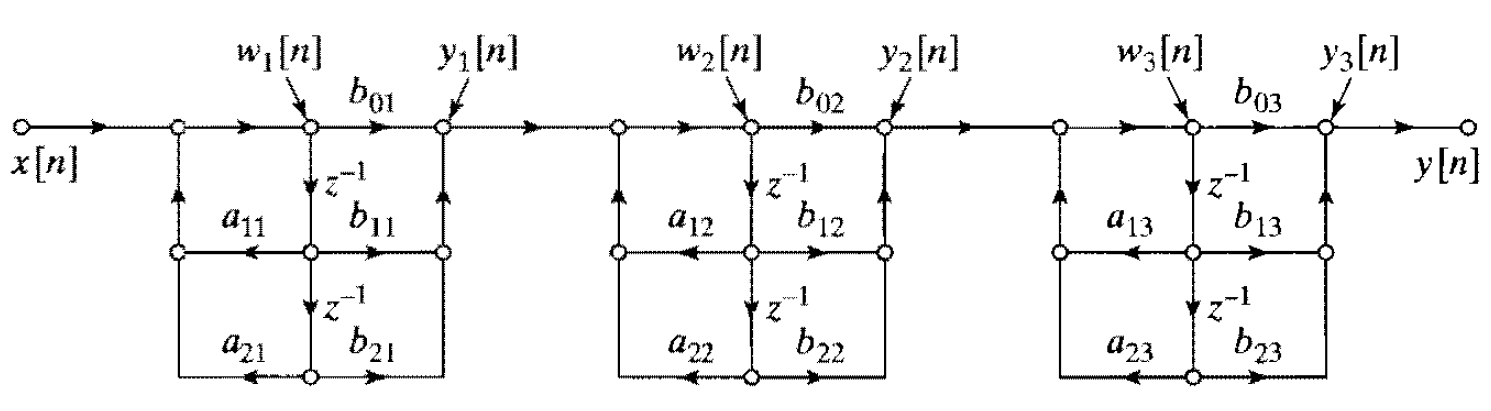
\includegraphics{figs/IIR_cascade_form.png}};
	\node[below, black, fill=black!20, scale=3] at ($(img1.south west)!0.2!(img1.south east)$) {$H_1(z)$};
	\node[below, black, fill=black!20, scale=3] at ($(img1.south west)!0.5!(img1.south east)$) {$H_2(z)$};
	\node[below, black, fill=black!20, scale=3] at ($(img1.south west)!0.8!(img1.south east)$) {$H_3(z)$};
	\end{tikzpicture}
	}
\end{center}

This figure shows a 6th-order system factored into three 2nd-order subsystems. Each subsystem is realized according to direct form II.
\end{frame}

\begin{frame}{Parallel forms}
	Now the factorization is done using \textbf{partial fraction expansion} of $H(z)$:
	
	\begin{equation*}
	H(z) = H_1(z) + H_2(z) + \ldots + H_K(z)
	\end{equation*}
	
	The subsystems $H_k(z), k = 1, \ldots, K$ are obtained by grouping second-order factors. These subsystems will either be simple delays or second-order systems:
	
	\begin{equation*}
	H_k(z) = \begin{cases}
	C_kz^{-k}, & \text{delay} \\
	\displaystyle\frac{e_{0k} + e_{1k}z^{-1}}{1 - a_{1k}z^{-1} + a_{2k}z^{-2}}, & \text{2nd-order system}
	\end{cases}, k = 1,\ldots, K
	\end{equation*}
	
	For partial fraction expansion use the Matlab function \texttt{residuez}
\end{frame}

\begin{frame}{Transposed forms}
	Transposed forms are obtained by performing \textbf{flow graph reversal} or \textbf{transposition}.

	In essence flow graph transposition is done by 
	\begin{enumerate}
		\item reversing all branches without changing the gain (transmittance) of each branch
		\item reversing the roles of input and output
	\end{enumerate}

	 For single-input single-output systems these operations do not change the system function as long as the input and output nodes are interchanged. 
\end{frame}

\begin{frame}{Transposed direct form I}
	\begin{columns}
		\begin{column}{0.5\textwidth}
			\textbf{Direct form I}
			\begin{center}
				\resizebox{\textwidth}{!}{\begin{tikzpicture}[node distance=2cm]
%Place the nodes
\node[terminal={below}{$x[n]$}] (x) at (0,0) {};
\node[terminal={below}{}, right of=x] (00) {};
\node[terminal={below}{}, right=2cm of 00] (01) {};
\node[terminal={below}{}, right of=01] (02) {};
\node[terminal={below}{}, right=2cm of 02] (03) {};
\node[terminal={below}{$\tikz[baseline]{\node[fill=blue!20,anchor=base] {$y[n]$};}$}, right of=03] (y) {};

\foreach \j in {1, 2} {
	\pgfmathtruncatemacro{\jn}{(\j-1)}%
	\node[terminal={left}{$x[n-\j]$}, below of=\jn0] (\j0) {};
	\node[terminal={left}{}, below of=\jn1] (\j1) {};
	\node[terminal={left}{}, below of=\jn2] (\j2) {};
	\node[terminal={right}{$y[n-\j]$}, below of=\jn3] (\j3) {};
	\draw[amark={$z^{-1}$}{left}] (\jn0) to (\j0);
	\draw[amark={$b_\jn$}{above}] (\jn0) to (\jn1);
	\draw[amark={}{left}] (\j1) to (\jn1);
	\draw[amark={}{left}] (\j2) to (\jn2);
	\draw[amark={$z^{-1}$}{right}] (\jn3) to (\j3);
	\draw[amark={$a_\j$}{above}] (\j3) to (\j2);
}

\node[terminal={left}{$x[n-N+1]$}, below=2.5cm of 20] (30) {};
\node[terminal={left}{$x[n-N]$}, below of=30] (40) {};
\node[terminal={left}{}, below=2.5cm of 21] (31) {};
\coordinate[below of=31] (41) {};

\draw[\thickness, dashed] (20) to (30);
\draw[\thickness, dashed] (21) to (31);
\draw[amark={$z^{-1}$}{left}] (30) to (40);
\draw[amark={$b_2$}{above}] (20) to (21);
\draw[amark={$b_{N-1}$}{above}] (30) to (31);
\draw[amark={$b_{N}$}{above}] (40) to (41);
\draw[\thickness] (41) to (31);

\node[terminal={right}{$y[n-N+1]$}, below=2.5cm of 23] (33) {};
\node[terminal={right}{$y[n-N]$}, below of=33] (43) {};
\node[terminal={left}{}, below=2.5cm of 22] (32) {};
\coordinate[below of=32] (42) {};

\draw[\thickness, dashed] (23) to (33);
\draw[\thickness, dashed] (22) to (32);
\draw[amark={$z^{-1}$}{right}] (33) to (43);
\draw[amark={$a_{N-1}$}{above}] (33) to (32);
\draw[amark={$a_{N}$}{above}] (43) to (42);
\draw[\thickness] (42) to (32);

\draw[amark={}{right}] (x) to (00);
\draw[amark={}{right}] (01) to (02);
\draw[amark={}{right}] (03) to (y);

\draw[amark={$1$}{above}] (02) to (03);
\node[above] at ($(01.north)$) {$\tikz[baseline]{\node[fill=blue!10,anchor=base] {$v[n]$};}$};

\node[below=0.1cm] at ($(40)!0.5!(41)$) {(zeros)};
\node[below=0.1cm] at ($(42)!0.5!(43)$) {(poles)};

\end{tikzpicture}}
			\end{center}
		\end{column}
		\begin{column}{0.5\textwidth}
			\textbf{Transposed direct form I}
			\begin{center}
				\resizebox{\textwidth}{!}{\begin{tikzpicture}[node distance=2cm]
%Place the nodes
\node[terminal={below}{$x[n]$}] (x) at (0,0) {};
\node[terminal={below}{}, right of=x] (00) {};
\node[terminal={below}{}, right=2cm of 00] (01) {};
\node[terminal={below}{}, right of=01] (02) {};
\node[terminal={below}{}, right=2cm of 02] (03) {};
\node[terminal={below}{$\tikz[baseline]{\node[fill=blue!20,anchor=base] {$y[n]$};}$}, right of=03] (y) {};

\foreach \j in {1, 2} {
	\pgfmathtruncatemacro{\jn}{(\j-1)}%
	\node[terminal={left}{}, below of=\jn0] (\j0) {};
	\node[terminal={left}{}, below of=\jn1] (\j1) {};
	\node[terminal={left}{}, below of=\jn2] (\j2) {};
	\node[terminal={right}{}, below of=\jn3] (\j3) {};
	\draw[amark={$z^{-1}$}{left}] (\j0) to (\jn0);
	\draw[amark={$a_\j$}{above}] (\j1) to (\j0);
	\draw[amark={$b_\jn$}{above}] (\j2) to (\j3);
	\draw[amark={}{left}] (\jn1) to (\j1);
	\draw[amark={}{left}] (\jn2) to (\j2);
	\draw[amark={$z^{-1}$}{right}] (\j3) to (\jn3);
}

\node[terminal={left}{}, below=2.5cm of 20] (30) {};
\node[terminal={left}{}, below of=30] (40) {};
\node[terminal={left}{}, below=2.5cm of 21] (31) {};
\coordinate[below of=31] (41) {};

\draw[\thickness, dashed] (20) to (30);
\draw[\thickness, dashed] (21) to (31);
\draw[amark={$z^{-1}$}{left}] (40) to (30);
\draw[amark={$a_{N-1}$}{above}] (31) to (30);
\draw[amark={$a_{N}$}{above}] (41) to (40);
\draw[\thickness] (41) to (31);

\node[terminal={right}{}, below=2.5cm of 23] (33) {};
\node[terminal={right}{}, below of=33] (43) {};
\node[terminal={left}{}, below=2.5cm of 22] (32) {};
\coordinate[below of=32] (42) {};

\draw[\thickness, dashed] (23) to (33);
\draw[\thickness, dashed] (22) to (32);
\draw[amark={$z^{-1}$}{right}] (43) to (33);
\draw[amark={$b_{N-1}$}{above}] (32) to (33);
\draw[amark={$b_{N}$}{above}] (42) to (43);
\draw[\thickness] (42) to (32);

\draw[amark={}{right}] (x) to (00);
\draw[amark={}{right}] (01) to (02);
\draw[amark={}{right}] (03) to (y);

\draw[amark={$b_0$}{above}] (02) to (03);
\draw[amark={$1$}{above}] (00) to (01);
\node[above] at ($(01.north)$) {$\tikz[baseline]{\node[fill=blue!10,anchor=base] {$v_T[n]$};}$};

\node[below=0.1cm] at ($(40)!0.5!(41)$) {(poles)};
\node[below=0.1cm] at ($(42)!0.5!(43)$) {(zeros)};

\end{tikzpicture}}
			\end{center}
		\end{column}
	\end{columns}
\end{frame}


\begin{frame}{Transposed direct form II}
	\begin{columns}[t]
		\begin{column}{0.5\textwidth}
			\textbf{Direct form II}
			\begin{center}
				\resizebox{\textwidth}{!}{\begin{tikzpicture}[node distance=1.75cm]
%Place the nodes
\node[terminal={below}{$x[n]$}] (x) at (0,0) {};
\node[terminal={below}{}, right of=x] (00) {};
\node[terminal={below}{}, right of= 00] (01) {};
\node[terminal={below}{}, right of=01] (02) {};
\node[terminal={below}{$\tikz[baseline]{\node[fill=blue!20,anchor=base] {$y[n]$};}$}, right of=02] (y) {};

\foreach \j in {1, 2, 3} {
	\pgfmathtruncatemacro{\jn}{(\j-1)}%
	\node[terminal={below}{}, below of=\jn0] (\j0) {};
	\node[terminal={below}{}, below of=\jn1] (\j1) {};
	\node[terminal={below}{}, below of=\jn2] (\j2) {};
}

\coordinate[below of=30] (40) {};
\coordinate[below of=32] (42) {};
\node[terminal={below}{}, below of=31] (41) {};

\node[above] (w) at (01) {$\tikz[baseline]{\node[fill=blue!10,anchor=base] {$w[n]$};}$};

%
\draw[zpath={right}] (01) to (11);
\draw[zpath={right}] (11) to (21);
\draw[\thickness, dashed] (21) to (31);
\draw[zpath={right}] (31) to (41);

%
\draw[amark] (10) to (00);
\draw[amark] (20) to (10);
\draw[\thickness, solid] (40) to (30);
\draw[\thickness, dashed] (30) to (20);

%
\draw[amark] (12) to (02);
\draw[amark] (22) to (12);
\draw[\thickness, solid] (42) to (32);
\draw[\thickness, dashed] (32) to (22);

%
\draw[amark={$1$}{above}] (00) to (01);
\draw[amark={$a_1$}{above}] (11) to (10);
\draw[amark={$a_2$}{above}] (21) to (20);
\draw[amark={$a_{N-1}$}{above}] (31) to (30);
\draw[amark={$a_N$}{above}] (41) to (40);

%
\draw[amark={$b_0$}{above}] (01) to (02);
\draw[amark={$b_1$}{above}] (11) to (12);
\draw[amark={$b_2$}{above}] (21) to (22);
\draw[amark={$b_{N-1}$}{above}] (31) to (32);
\draw[amark={$b_N$}{above}] (41) to (42);


\draw[amark] (x) to (00);
\draw[amark] (02) to (y);

\node[below] at ($(40)!0.5!(41)$) {(poles)};
\node[below] at ($(41)!0.5!(42)$) {(zeros)};

\end{tikzpicture}}
			\end{center}
		\end{column}
		\begin{column}{0.5\textwidth}
			\textbf{Transposed direct form II}
			\begin{center}
				\resizebox{\textwidth}{!}{\begin{tikzpicture}[node distance=1.75cm]
%Place the nodes
\node[terminal={below}{$x[n]$}] (x) at (0,0) {};
\node[terminal={below}{}, right of=x] (00) {};
\node[terminal={below}{}, right of= 00] (01) {};
\node[terminal={below}{}, right of=01] (02) {};
\node[terminal={below}{$\tikz[baseline]{\node[fill=blue!20,anchor=base] {$y[n]$};}$}, right of=02] (y) {};

\foreach \j in {1, 2, 3} {
	\pgfmathtruncatemacro{\jn}{(\j-1)}%
	\node[terminal={below}{}, below of=\jn0] (\j0) {};
	\node[terminal={below}{}, below of=\jn1] (\j1) {};
	\node[terminal={below}{}, below of=\jn2] (\j2) {};
}

\coordinate[below of=30] (40) {};
\coordinate[below of=32] (42) {};
\node[terminal={below}{}, below of=31] (41) {};

\node[above] (w) at (01) {$\tikz[baseline]{\node[fill=blue!10,anchor=base] {$w_T[n]$};}$};

%
\draw[zpath={right}] (11) to (01);
\draw[zpath={right}] (21) to (11);
\draw[\thickness, dashed] (31) to (21);
\draw[zpath={right}] (41) to (31);

%
\draw[amark] (00) to (10);
\draw[amark] (10) to (20);
\draw[\thickness, solid] (30) to (40);
\draw[\thickness, dashed] (20) to (30);

%
\draw[amark] (02) to (12);
\draw[amark] (12) to (22);
\draw[\thickness, solid] (32) to (42);
\draw[\thickness, dashed] (22) to (32);

%
\draw[amark={$b_0$}{above}] (00) to (01);
\draw[amark={$b_1$}{above}] (10) to (11);
\draw[amark={$b_2$}{above}] (20) to (21);
\draw[amark={$b_{N-1}$}{above}] (30) to (31);
\draw[amark={$b_N$}{above}] (40) to (41);

%
\draw[amark={$1$}{above}] (01) to (02);
\draw[amark={$a_1$}{above}] (12) to (11);
\draw[amark={$a_2$}{above}] (22) to (21);
\draw[amark={$a_{N-1}$}{above}] (32) to (31);
\draw[amark={$a_N$}{above}] (42) to (41);


\draw[amark] (x) to (00);
\draw[amark] (02) to (y);

\node[below] at ($(40)!0.5!(41)$) {(zeros)};
\node[below] at ($(41)!0.5!(42)$) {(poles)};

\end{tikzpicture}}
			\end{center}
			\pause
			Used in Matlab's \texttt{filter} function
		\end{column}
	\end{columns}
\end{frame}

\section{Structures for FIR Systems}
\begin{frame}<beamer:1|handout:0>{Outline}
\tableofcontents[currentsection]
\end{frame}

\begin{frame}{Structures for FIR systems}
FIR systems do not have the autoregressive component (no feedback). 

The \textbf{direct form I} simply realizes the convolution sum
\begin{equation*}
H(z) = \sum_{k = 0}^Mb_kz^{-k} = \sum_{k = 0}^M h[k]z^{-k}
\end{equation*}

\begin{center}
	\resizebox{\textwidth}{!}{\begin{tikzpicture}[node distance=1.75cm]
%Place the nodes
\node[terminal={below}{$x[n]$}] (x) at (0,0) {};
\node[terminal={below}{}, right of=x] (00) {};
\node[terminal={below}{}, right of= 00] (01) {};
\node[terminal={below}{}, right of=01] (02) {};
\node[terminal={below}{}, right of=02] (03) {};
\node[terminal={below}{}, right of=03] (04) {};

\coordinate[below of=00] (10) {};
\node[terminal={below}{}, right of=10] (11) {};
\node[terminal={below}{}, right of=11] (12) {};
\node[terminal={below}{}, right of=12] (13) {};
\node[terminal={below}{}, right of=13] (14) {};
\node[terminal={below}{$y[n]$}, right of=14] (y) {};

\foreach \l [count=\j]  in {$h[0]$, $h[1]$, $h[2]$, $h[M-1]$} {
	\pgfmathtruncatemacro{\jn}{(\j-1)}%
	\ifthenelse{\j = 3}
		{\draw[\thickness, dashed] (0\jn) to (0\j)}
		{\draw[zpath={above}] (0\jn) to (0\j)};
	\ifthenelse{\j = 3}
		{\draw[\thickness, dashed] (1\jn) to (1\j)}
		{\draw[amark={}{right}] (1\jn) to (1\j)};
	%\draw[zpath={above}] (0\jn) to (0\j);
	\draw[amark={\l}{right}] (0\jn) to (1\jn);
	
}

\draw[amark={$h[M]$}{right}] (04) to (14);
\draw[amark={}{right}] (14) to (y);

\draw[amark] (x) to (00);
\draw[amark] (14) to (y);

\end{tikzpicture}}
\end{center}

This operation is commonly called\textbf{ multiply-accumulate (MAC)}

\end{frame}

\begin{frame}{FIR transposed direct form}
Similarly to IIR structures, we can apply flow graph transposition to obtain the transposed forms

\textbf{Direct form}
\begin{center}
	\resizebox{0.9\textwidth}{!}{\begin{tikzpicture}[node distance=1.75cm]
%Place the nodes
\node[terminal={below}{$x[n]$}] (x) at (0,0) {};
\node[terminal={below}{}, right of=x] (00) {};
\node[terminal={below}{}, right of= 00] (01) {};
\node[terminal={below}{}, right of=01] (02) {};
\node[terminal={below}{}, right of=02] (03) {};
\node[terminal={below}{}, right of=03] (04) {};

\coordinate[below of=00] (10) {};
\node[terminal={below}{}, right of=10] (11) {};
\node[terminal={below}{}, right of=11] (12) {};
\node[terminal={below}{}, right of=12] (13) {};
\node[terminal={below}{}, right of=13] (14) {};
\node[terminal={below}{$y[n]$}, right of=14] (y) {};

\foreach \l [count=\j]  in {$h[0]$, $h[1]$, $h[2]$, $h[M-1]$} {
	\pgfmathtruncatemacro{\jn}{(\j-1)}%
	\ifthenelse{\j = 3}
		{\draw[\thickness, dashed] (0\jn) to (0\j)}
		{\draw[zpath={above}] (0\jn) to (0\j)};
	\ifthenelse{\j = 3}
		{\draw[\thickness, dashed] (1\jn) to (1\j)}
		{\draw[amark={}{right}] (1\jn) to (1\j)};
	%\draw[zpath={above}] (0\jn) to (0\j);
	\draw[amark={\l}{right}] (0\jn) to (1\jn);
	
}

\draw[amark={$h[M]$}{right}] (04) to (14);
\draw[amark={}{right}] (14) to (y);

\draw[amark] (x) to (00);
\draw[amark] (14) to (y);

\end{tikzpicture}}
\end{center}

\textbf{Transposed direct form}
\begin{center}
	\resizebox{0.9\textwidth}{!}{\begin{tikzpicture}[node distance=1.75cm]
%Place the nodes
\node[terminal={below}{$x[n]$}] (x) at (0,0) {};
\node[terminal={below}{}, right of=x] (10) {};
\node[terminal={below}{}, above of=10] (00) {};
\node[terminal={below}{}, right of= 00] (01) {};
\node[terminal={below}{}, right of=01] (02) {};
\node[terminal={below}{}, right of=02] (03) {};
\node[terminal={below}{}, right of=03] (04) {};

\node[terminal={below}{}, right of=10] (11) {};
\node[terminal={below}{}, right of=11] (12) {};
\node[terminal={below}{}, right of=12] (13) {};
\node[terminal={below}{}, right of=13] (14) {};
\node[terminal={below}{$y[n]$}, right of=04] (y) {};

\foreach \l [count=\j]  in {$h[0]$, $h[1]$, $h[2]$, $h[M-1]$} {
	\pgfmathtruncatemacro{\jn}{(\j-1)}%
	\ifthenelse{\j = 3}
		{\draw[\thickness, dashed] (0\jn) to (0\j)}
		{\draw[zpath={above}] (0\jn) to (0\j)};
	\ifthenelse{\j = 3}
		{\draw[\thickness, dashed] (1\jn) to (1\j)}
		{\draw[amark={}{right}] (1\jn) to (1\j)};
	%\draw[zpath={above}] (0\jn) to (0\j);
	\draw[amark={\l}{right}] (1\jn) to (0\jn);
	
}

\draw[amark={$h[M]$}{right}] (14) to (04);
\draw[amark={}{right}] (04) to (y);

\draw[amark] (x) to (10);

\end{tikzpicture}}
\end{center}

\end{frame}

\begin{frame}{FIR linear phase systems}
The impulse response of FIR linear phase systems have either even or odd symmetry

We can \underline{halve} the number of multiplications by leveraging this symmetry
~\\
~\\
\textbf{Example:} Direct form of a \textbf{type I filter} (even symmetry and $M$ even)
\begin{columns}
	\begin{column}{0.7\textwidth}
		\begin{center}
			\resizebox{\textwidth}{!}{\begin{tikzpicture}[node distance=1.75cm]
%Place the nodes
\node[terminal={below}{$x[n]$}] (x) at (0,0) {};
\node[terminal={below}{}, right of=x] (00) {};
\node[terminal={below}{}, right of= 00] (01) {};
\node[terminal={below}{}, right of=01] (02) {};
\node[terminal={below}{}, right of=02] (03) {};
\coordinate[right of=03] (04) {};

\coordinate[below=3cm of 00] (20) {};
\node[terminal={below}{}, below=3cm of 00] (21) {};
\node[terminal={below}{}, below=3cm of 01] (22) {};
\node[terminal={below}{}, below=3cm of 02] (23) {};
\node[terminal={below}{}, below=3cm of 03] (24) {};
\node[terminal={below}{}, right of=24] (25) {};

\node[terminal={below}{}] (11) at ($(00)!0.5!(20) - (1cm, 0)$) {};
\node[terminal={below}{}, right of=11] (12) {};
\node[terminal={below}{}, right of=12] (13) {};
\node[terminal={below}{}, right of=13] (14) {};

\node[terminal={below}{}, below=3cm of 11] (31) {};
\node[terminal={below}{}, below=3cm of 12] (32) {};
\node[terminal={below}{}, below=3cm of 13] (33) {};
\node[terminal={below}{}, below=3cm of 14] (34) {};
\node[terminal={below}{$y[n]$}] (y) at (31 -| x) {};

\coordinate (35) at (34 -| 25) {};


\foreach \l [count=\j]  in {$h[0]$, $h[1]$, $h[2]$, $h[M/2-1]$} {
	\pgfmathtruncatemacro{\jn}{(\j-1)}%
	\ifthenelse{\j = 3}
		{\draw[\thickness, dashed] (0\jn) to (0\j)}
		{\draw[zpath={above}] (0\jn) to (0\j)};
	\ifthenelse{\j = 4}
		{\draw[\thickness, dashed] (2\j) to (2\jn)}
		{\draw[earlymark={$z^{-1}$}{below}] (2\j) to (2\jn)};
	%\draw[zpath={above}] (0\jn) to (0\j);
	\draw[latemark={\l}{right}] (1\j) to (3\j);
	\draw[amark={}{right}] (0\jn) to (1\j);	
	\draw[amark={}{right}] (2\j) to (1\j);
}

\draw[\thickness, solid] (04) to (25);
\draw[zpath={below}] (25) to (24);
\draw[amark={$h[M/2]$}{right}] (25) to (35);

\draw[\thickness, solid] (35) to (34);
\draw[\thickness, dashed] (34) to (33);
\draw[amark={}{right}] (33) to (32);
\draw[amark={}{right}] (32) to (31);
\draw[amark={}{right}] (31) to (y);


%\draw[amark={$h[M]$}{right}] (14) to (04);
%\draw[amark={}{right}] (14) to (y);

\draw[amark] (x) to (00);
%\draw[amark] (14) to (y);

\end{tikzpicture}}
		\end{center}
	\end{column}


	\begin{column}{0.4\textwidth}
	\begin{center}
		\resizebox{\textwidth}{!}{
			\begin{tikzpicture} 
			\begin{axis}[
			axis lines*=middle, 
			enlargelimits = true, clip=false,
			ymin=0, %ymax=1.2,
			hide y axis,
			xmin=0, xmax=15,
			axis line style={->,>=stealth},
			xlabel={$n$},
			every axis x label/.style={
				at={(ticklabel* cs:1)},
				anchor=west,
			},
			ytick=\empty, xtick={0.01,8,16},
			xticklabels={$0$, $M/2$, $M$},
			every outer y axis line/.append style={white!15!black},
			every y tick label/.append style={font=\color{white!15!black}},
			legend style={draw=white!15!black,fill=white,legend cell align=left}]
			\addplot[ycomb, mark=*, fill=white, mark options={scale=1.5, fill=white}, line width=1.5pt, domain=0:16, samples=17] {sinc((x-8)/3)};

			\node[above] at (axis cs: 0, 0.1) {$h[0]$};
			\node[above] at (axis cs: 8, 1) {$h[M/2]$};
			
			\end{axis}
			\end{tikzpicture}
		}
	\end{center}
	\end{column}
\end{columns}

Only the samples $h[0], \ldots, h[M/2]$ are used in the implementation

\end{frame}

\section{Pipelining and Parallel Processing}
\begin{frame}<beamer:1|handout:0>{Outline}
\tableofcontents[currentsection]
\end{frame}

\begin{frame}{Pipelining and parallel processing}
\textbf{Question:} how to implement this filter for a signal of rate $1/T = 1$ GHz when the multiplications are performed at $1/T_M = 100$ MHz?

\begin{center}
	\resizebox{0.9\textwidth}{!}{\begin{tikzpicture}[node distance=1.75cm]
%Place the nodes
\node[terminal={below}{$x[n]$}] (x) at (0,0) {};
\node[terminal={below}{}, right of=x] (00) {};
\node[terminal={below}{}, right of= 00] (01) {};
\node[terminal={below}{}, right of=01] (02) {};
\node[terminal={below}{}, right of=02] (03) {};
\node[terminal={below}{}, right of=03] (04) {};

\coordinate[below of=00] (10) {};
\node[terminal={below}{}, right of=10] (11) {};
\node[terminal={below}{}, right of=11] (12) {};
\node[terminal={below}{}, right of=12] (13) {};
\node[terminal={below}{}, right of=13] (14) {};
\node[terminal={below}{$y[n]$}, right of=14] (y) {};

\foreach \l [count=\j]  in {$h[0]$, $h[1]$, $h[2]$, $h[M-1]$} {
	\pgfmathtruncatemacro{\jn}{(\j-1)}%
	\ifthenelse{\j = 3}
		{\draw[\thickness, dashed] (0\jn) to (0\j)}
		{\draw[zpath={above}] (0\jn) to (0\j)};
	\ifthenelse{\j = 3}
		{\draw[\thickness, dashed] (1\jn) to (1\j)}
		{\draw[amark={}{right}] (1\jn) to (1\j)};
	%\draw[zpath={above}] (0\jn) to (0\j);
	\draw[amark={\l}{right}] (0\jn) to (1\jn);
	
}

\draw[amark={$h[M]$}{right}] (04) to (14);
\draw[amark={}{right}] (14) to (y);

\draw[amark] (x) to (00);
\draw[amark] (14) to (y);

\end{tikzpicture}}
\end{center}

Two solutions:
\begin{enumerate}
	\item Pipelining
	\item Parallel processing
\end{enumerate}

Pipelining and parallel processing solve the problem in two complementary ways. Hence, they can be use together, which is generally done in practice. 

\end{frame}

\begin{frame}{Pipelining}
Suppose we want to implement this 3-tap FIR filter in real time. 

\begin{center}
	\resizebox{0.7\textwidth}{!}{\begin{tikzpicture}[node distance=1.75cm]
%Place the nodes
\node[terminal={below}{$x[n]$}] (x) at (0,0) {};
\node[terminal={below}{}, right of=x] (00) {};
\node[terminal={below}{}, right of= 00] (01) {};
\node[terminal={below}{}, right of= 01] (02) {};


\coordinate[below of=00] (10) {};
\node[terminal={below}{}, right of=10] (11) {};
\node[terminal={below}{}, right of=11] (12) {};

\draw[zpath={above}] (00) to (01);
\draw[zpath={above}] (01) to (02);

\draw[amark={$h_0$}{right}, red2] (00) to (10);
\draw[amark={$h_1$}{right}] (01) to (11);


\draw[amark, red2] (10) to (11);
\draw[amark, red2] (11) to (12);

\draw[amark, red2] (x) to (00);


\ifdefined\PIPE
	\node[terminal={below}{}, right of= 02] (03) {};
	\node[terminal={below}{}, right of=12] (13) {};
	\node[terminal={below}{$y[n]$}, right of=13] (y) {};
	
	\draw[zpath={above}] (02) to (03);
	\draw[zpath={above}] (12) to (13);
	\draw[amark={$h_2$}{right}] (03) to (13);
	
	\draw[amark] (13) to (y);
	
	\draw[dashed] ($(02)+(0.25cm, 0.6cm)$) rectangle ($(13)-(0.25cm, 0.1cm)$);
	\node[above] at ($(02)!0.5!(03) + (0, 0.6cm)$) {Added memory}; 
	
	\node[below left, blue2] at (12) {1};
	\node[below left, blue2] at (13) {2};
	\node[above right, blue2] at (13) {3};
	
\else
	\node[terminal={below}{$y[n]$}, right of=12] (y) {};
	\draw[amark, red2] (12) to (y);
	
	\draw[amark={$h_2$}{right}] (02) to (12);
\fi


\end{tikzpicture}}
\end{center}

The {\color{red2} \textbf{critical path}} of this filter has one multiplication, which takes $T_M$ seconds, and two additions, which take $T_A$ seconds each

Therefore the sampling period $T$ should satisfy
\begin{equation*}
T > T_M + 2T_A,
\end{equation*}
so that all operations in the critical path will have been finished by the time a new input sample comes in.

\pause
\textbf{Question:} what can we do if $T < T_M + 2T_A$ i.e., operations are too slow? 
\end{frame}

\begin{frame}{Pipelining}
\textbf{Solution:} add memory $z^{-1}$
\begin{center}
	\def\PIPE{1}
	\resizebox{0.8\textwidth}{!}{\begin{tikzpicture}[node distance=1.75cm]
%Place the nodes
\node[terminal={below}{$x[n]$}] (x) at (0,0) {};
\node[terminal={below}{}, right of=x] (00) {};
\node[terminal={below}{}, right of= 00] (01) {};
\node[terminal={below}{}, right of= 01] (02) {};


\coordinate[below of=00] (10) {};
\node[terminal={below}{}, right of=10] (11) {};
\node[terminal={below}{}, right of=11] (12) {};

\draw[zpath={above}] (00) to (01);
\draw[zpath={above}] (01) to (02);

\draw[amark={$h_0$}{right}, red2] (00) to (10);
\draw[amark={$h_1$}{right}] (01) to (11);


\draw[amark, red2] (10) to (11);
\draw[amark, red2] (11) to (12);

\draw[amark, red2] (x) to (00);


\ifdefined\PIPE
	\node[terminal={below}{}, right of= 02] (03) {};
	\node[terminal={below}{}, right of=12] (13) {};
	\node[terminal={below}{$y[n]$}, right of=13] (y) {};
	
	\draw[zpath={above}] (02) to (03);
	\draw[zpath={above}] (12) to (13);
	\draw[amark={$h_2$}{right}] (03) to (13);
	
	\draw[amark] (13) to (y);
	
	\draw[dashed] ($(02)+(0.25cm, 0.6cm)$) rectangle ($(13)-(0.25cm, 0.1cm)$);
	\node[above] at ($(02)!0.5!(03) + (0, 0.6cm)$) {Added memory}; 
	
	\node[below left, blue2] at (12) {1};
	\node[below left, blue2] at (13) {2};
	\node[above right, blue2] at (13) {3};
	
\else
	\node[terminal={below}{$y[n]$}, right of=12] (y) {};
	\draw[amark, red2] (12) to (y);
	
	\draw[amark={$h_2$}{right}] (02) to (12);
\fi


\end{tikzpicture}}
\end{center}

By adding the extra memory the function of the filter is not altered. However, now the {\color{red2} \textbf{critical path}} only has one multiplication and one addition. 


Therefore, if

\begin{equation*}
T > T_M + T_A, 
\end{equation*}

the value at {\color{blue2} node 1} will be stored in the memory by the time a new input sample comes in. Hence, the first part of the circuit can start \textit{working} on the new sample, while the second part still \textit{works} on the previous sample.

\end{frame}


\begin{frame}
The pipelined FIR filter has the following \textit{schedule} assuming $T > T_M + T_A$ 

\begin{center}
	\def\PIPE{1}
	\resizebox{0.8\textwidth}{!}{\begin{tikzpicture}[node distance=1.75cm]
%Place the nodes
\node[terminal={below}{$x[n]$}] (x) at (0,0) {};
\node[terminal={below}{}, right of=x] (00) {};
\node[terminal={below}{}, right of= 00] (01) {};
\node[terminal={below}{}, right of= 01] (02) {};


\coordinate[below of=00] (10) {};
\node[terminal={below}{}, right of=10] (11) {};
\node[terminal={below}{}, right of=11] (12) {};

\draw[zpath={above}] (00) to (01);
\draw[zpath={above}] (01) to (02);

\draw[amark={$h_0$}{right}, red2] (00) to (10);
\draw[amark={$h_1$}{right}] (01) to (11);


\draw[amark, red2] (10) to (11);
\draw[amark, red2] (11) to (12);

\draw[amark, red2] (x) to (00);


\ifdefined\PIPE
	\node[terminal={below}{}, right of= 02] (03) {};
	\node[terminal={below}{}, right of=12] (13) {};
	\node[terminal={below}{$y[n]$}, right of=13] (y) {};
	
	\draw[zpath={above}] (02) to (03);
	\draw[zpath={above}] (12) to (13);
	\draw[amark={$h_2$}{right}] (03) to (13);
	
	\draw[amark] (13) to (y);
	
	\draw[dashed] ($(02)+(0.25cm, 0.6cm)$) rectangle ($(13)-(0.25cm, 0.1cm)$);
	\node[above] at ($(02)!0.5!(03) + (0, 0.6cm)$) {Added memory}; 
	
	\node[below left, blue2] at (12) {1};
	\node[below left, blue2] at (13) {2};
	\node[above right, blue2] at (13) {3};
	
\else
	\node[terminal={below}{$y[n]$}, right of=12] (y) {};
	\draw[amark, red2] (12) to (y);
	
	\draw[amark={$h_2$}{right}] (02) to (12);
\fi


\end{tikzpicture}}
\end{center}

\begin{center}
	\resizebox{\textwidth}{!}{
\begin{tabular}{cccccc}
	Time & Input & {\color{blue2} Node 1} & {\color{blue2} Node 2} & {\color{blue2} Node 3} & Output \\
	\hline
	0 & $x[0]$ & $h_0x[0] + h_1x[-1]$ & - & - & - \\ \pause
	T & $x[1]$ & $h_0x[1] + h_1x[0]$ & $h_0x[0] + h_1x[-1]$ & $h_2x[-2]$ & $y[0]$ \\ \pause
	2T & $x[2]$ & $h_0x[2] + h_1x[1]$ & $h_0x[1] + h_1x[0]$ & $h_2x[-1]$ & $y[1]$ \\ \pause
	3T & $x[3]$ & $h_0x[3] + h_1x[2]$ & $h_0x[2] + h_1x[1]$ & $h_2x[0]$ & $y[2]$ \\
	\hline
\end{tabular}
}
\end{center}

\onslide<4|handout:1>{
Pipelining increases the \textbf{latency}. Note that the outputs are delayed by $1$ sample. That is, when the input is $x[1]$, the output will be $y[0]$, which corresponds to the input $x[0]$.
}
\end{frame}

\begin{frame}{Parallel processing}
Processes several inputs at the same time

This difference equation takes one input $x[n]$ and produces one output $y[n]$
\begin{equation*}
y[n] = h_0x[n] + h_1x[n-1] + h_2x[n-2]
\end{equation*}
\pause
We can rewrite it this way
\begin{align*}
y[3k] &= h_0x[3k] + h_1x[3k-1] + h_2x[3k-2] \\
y[3k+1] &= h_0x[3k+1] + h_1x[3k] + h_2x[3k-1] \\
y[3k+2] &= h_0x[3k+2] + h_1x[3k+1] + h_2x[3k]
\end{align*}

\begin{itemize}
	\item Now there are three inputs $\{x[3k], x[3k+1], x[3k+2]\}$ and three outputs $\{y[3k], y[3k+1], y[3k+2]\}$.
	\item Each difference equation is a FIR filter with the same coefficients as the original filter
	\item This can be extended to more inputs/outputs.
\end{itemize}
\end{frame}

\begin{frame}<beamer:0|handout:1>{Pipelining and parallel processing}
Additional comments

\begin{itemize}
	\item Pipelining and parallel processing solve the problem of using a slow hardware to process a fast signal in two complementary ways. 
	\item Pipelining solves the problem  by introducing memories and reducing the critical path. These memories are used to store ``partial results'', so that computations for new input samples can start before all the output has been calculated. The name pipeline comes from the analogy with a water pipe: ``continue sending water without waiting for the water in the pipe to come out.''
	\item Pipelining increases the latency and requires more memory
	\item Parallel processing solves the problem by processing multiple inputs simultaneously
	\item The effective speed of the hardware is increased by the level of parallelism
	\item The drawback of parallel processing is that we essentially have to replicate the hardware several times
\end{itemize}
\end{frame}


%
\begin{frame}{Summary}
\begin{itemize}
	\item There are different forms of realizing IIR and FIR rational systems
	\item Their difference becomes evident when considering finite arithmetic precision
	\item Pipelining and parallel processing solve the problem of using a slow hardware to process a fast signal in two complementary ways. 
	\item Pipelining adds memory (delays) to minimize the critical path. Consequently, pipelining increases latency
	\item In parallel processing the hardware is replicated to allow processing of multiple input samples simultaneously
	\item Pipelining and parallel processing can be realized together
	\item Pipelining and parallel processing are more difficult in IIR systems due to their inherent feedback
\end{itemize}
\end{frame}

\end{document}
